\chapter{Esettanulmány}

Az esettanulmányomnak a célja, hogy egy példán keresztül bemutassam az általam fejlesztett elemző eszköz valamint a rendszermodellből való származtatásnak a folyamatát.

Az esettanulmányom tárgyaként az elektronikus vezérlő egységek (ECU) diagnosztikai szolgáltatását választottam. Ennek oka egyrészről az, hogy az elemzett diagnosztikai szolgáltatások specifikációja publikusan elérhető az ISO 14229 "Road vehicles - Unified Diagnostic Services (UDS)" \cite{ISO14229} szabványban. Másrészről ez egy olyan potenciális belépőpontja lehet a támadóknak amely nem igényel semmiféle fizikai hozzáférést a járműhöz. Amennyiben távolról sikeresen hozzáfér és átveszi az irányítását a támadó egy elektronikus vezérlő egységnek, ami képes V2X vagy más vezetéknélküli szolgáltatásra, onnantól kezdve a jármű többi részén lévő diagnosztikai szolgáltatások is elérhetővé válhatnak számára.\\

Az ISO 14229\cite{ISO14229} definiálja az Unified Diagnostic Services (röviden UDS) protokollt ami egy alkalmazásrétegbeli szolgáltatás. Általános IT biztonsági szempontból, ehhez legközelebbinek a TLS és HTTPS protokollok lennének mondhatók.

\begin{figure}[!ht]
	\centering
	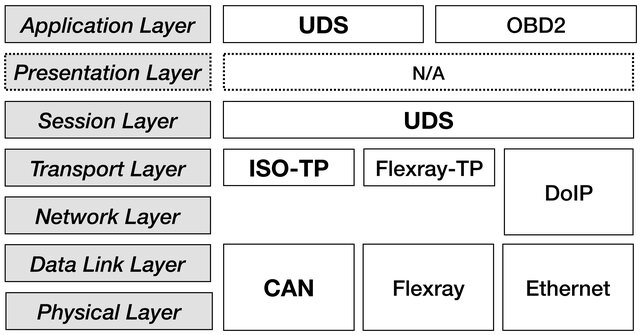
\includegraphics[width=130mm, keepaspectratio]{figures/06_isoosi.jpg}
	\caption{ISO/OSI modell autóipari kommunikációs protokollokra\cite{ISOOSI}}
\end{figure}

Az esettanulmányomban a szolgáltatások közül kettővel, a diagnosztikai autentikációval, valamint a software frissítéssel fogok foglalkozni, mivel ezek a kiemelten kiberbiztonsági relevanciával rendelkező szolgáltatások.\\

A diagnosztikai autentikációt két módon lehet implementálni. Az egyik a \textbf{Security Access (0x27)} a másik pedig a korszerűbb \textbf{Authentication (0x29)} lenne. 

A \textbf{Security Access}-szel az úgynevezett challange-response autentikációt lehet megvalósítani, amelynek a menete először egy valamilyen ismeretlen ECU-n belüli információnak (\textit{seed}) a szolgáltatása a diagnosztikai tesztelő részére, aki ezt az információt valamilyen közös titok (pl: szimmetrikus kulcs) használatával előállít egy kulcsot, amelyet elküld az ECU-nak. Az ECU a fogadó oldalon ellenőrzi, hogy a kulcs ami érkezett az megegyezik azzal amit ugyanezen közös titok és algoritmus használatával állított elő a \textit{seed} lekérése után. Amennyiben a kulcsok megegyeznek az ECU a felhasználót átengedi magasabb biztonsági szinthez ezzel hozzáférést biztosítva korábban nem elérhető diagnosztikai szolgáltatásokhoz.

Az \textbf{Authentication} már egy jóval komplexebb, tanúsítvány alapú autentikációt tesz lehetővé. Ennek a bemutatása túl mutat a jelen esettanulmányon.\\

A szoftverfrissítés egy több lépésből álló szekvenciája diagnosztikai rutin hívásoknak, amelyeket a szabvány "Upload download functional unit" fejezetében fejt ki.

Annak a folyamata, hogy egy új szoftver kerüljön fel az ECU-ra jellemzően a következő lépésekből áll:
\begin{itemize}
	\item \textbf{RequestDownload (0x34)}: Előfeltételek ellenőrzése, letöltési kérelem jóváhagyása
	\item \textbf{TransferData (0x36)}: Adatok feltöltése
	\item \textbf{RequestTransferExit (0x37)}: Érkezett adatok ellenőrzése, jóváhagyás, szoftver indíthatóvá tétele
\end{itemize}

Ezt a folyamat természetesen bővíthető további vagy ezeket megelőző lépésekkel, illetve az egyes rutinok belső működése sincs szabályozva. Maga a kerete viszont egy szoftverfrissítésnek az jellemzően ilyen diagnosztikai szolgáltatások futtatásával és kérések kiszolgálásával történnek az elektronikus vezérlőegységeken.

Érdemes kiemelni itt, hogy ez a frissítési metódus eleinte a járműszervizben történt volna a szerelő által, de a napjainkban már ezeknek a távoli elérése, jellemzően egy külön erre integrált elektronikus vezérlőegység által is lehet lefolytatva. Ezeknek sokban kényelmi, de szintén szoftveres sérülékenységek vagy hibák javítása szempontjából is fontos szerepük van.\\

A protokoll egyébként tartalmaz olyan szolgáltatásokat mint a \textbf{Routine Control (0x31)} amellyel a beszállító és a vevő az eszközre specifikus, nem szabványos diagnosztikai szolgáltatásokat is definiálhat. Ilyenek lehetnek kulcs és tanúsítványkezelő rutinok.

\section{Károkozások és értékek azonosítása}

A \ref{fig:diag_abuse} ábrán láthatóak a potenciális károkozások. A korábban meghatároztuk a két fő szolgáltatást ami az esettanulmányban elemzésre kerül, majd ezekhez a CIA triád mentén való elemzés szerint meghatározásra kerültek a potenciális károkozások. Továbbá egy egy azonosító is került a károkozások nevébe, valamint a felvett sztereotípiával az attributálást is el lehetett végezni.

\begin{itemize}
	\item \textbf{DS-SECDIAG-00 Leak confidential data}: Amennyiben az autentikációs szolgáltatás bizalmassága elveszik, abban az esetben a támadónak lehetősége lesz a bizalmas diagnosztikai adatok kiolvasására
	\item \textbf{DS-SECDIAG-01 Acces unauthorized functionality}: Az autentikációs szolgáltatás integritásának a megtörése vezethet olyan szolgáltatások elérhetővé válásához amelyek normális esetben nem lennének elérhetőek
	\item \textbf{DS-SECDIAG-02 Block authentication attempts}: Az autentikációs szolgáltatás elérhetőségének a blokkolásával korlátozható jogosult felhasználóknak a korlátozott szolgáltatásokhoz való hozzáférése
	\item \textbf{DS-SECSW-00 Leak software}: A szoftver kiszivárogtatásával lehetőség adódik a szoftverben sérülékenységek keresésére, annak kihasználását könnyebbé téve
	\item \textbf{DS-SECSW-01 Change software}: A szoftver megváltoztatásával kártékony szoftver is feljuttatható az elektronikus vezérlőegységre
	\item \textbf{DS-SECSW-02 Remove software}: A szoftver elérhetőségének korlátozásával az elektronikus vezérlőegység teljes funkcionalitása blokkolhatóvá tehető
\end{itemize}

\begin{figure}[!ht]
	\centering
	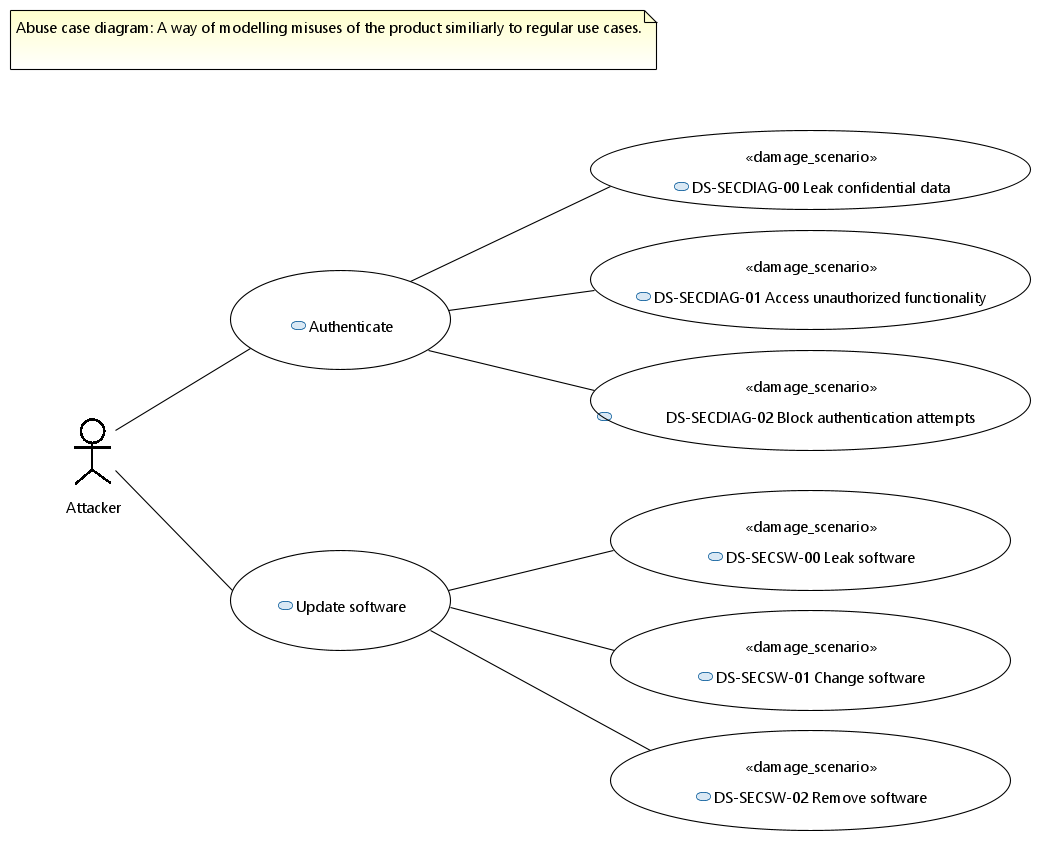
\includegraphics[width=130mm, keepaspectratio]{figures/06_01_abuse_case_diagram.PNG}
	\caption{Diagnosztika kihasználási esetei}
	\label{fig:diag_abuse}
\end{figure}

\begin{figure}[!ht]
	\centering
	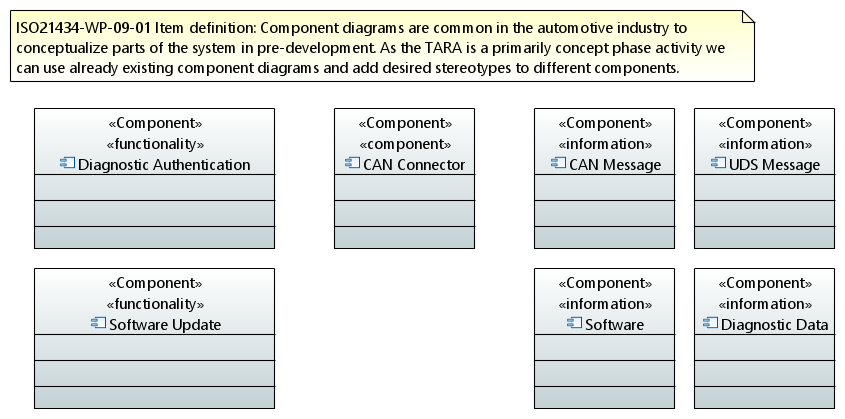
\includegraphics[width=130mm, keepaspectratio]{figures/06_02_item_definition_diagram.PNG}
	\caption{Diagnosztika termékleírása}
\end{figure}